\documentclass[12pt,a4paper]{book}

% Encoding & language
\usepackage[T1]{fontenc}
\usepackage[utf8]{inputenc}
\usepackage[indonesian]{babel}

% Page layout
\usepackage[a4paper,top=2.5cm,bottom=2.5cm,left=2.8cm,right=2.5cm]{geometry}

% Fonts
\usepackage{lmodern}

% Graphics
\usepackage{graphicx}
\graphicspath{{images/}}

% Colors and boxes
\usepackage[dvipsnames,svgnames,x11names]{xcolor}
\usepackage[most]{tcolorbox}

% Code listings
\usepackage{listings}

% Tables
\usepackage{booktabs}
\usepackage{longtable}
\usepackage{array}

% Headers/footers
\usepackage{fancyhdr}

% URL/path breaking
\usepackage[hyphens]{url}

% Misc
\usepackage{microtype}
\usepackage{enumitem}
\usepackage{emptypage}

% Allow extra stretch before declaring overfull
\setlength{\emergencystretch}{3em}

% Hyperlinks (load last)
\usepackage[hidelinks,unicode,
  pdftitle={Buku Manual PakAI},
  pdfauthor={Dian Hanifudin Subhi, Dhebys Suryani Hormansyah, Agung Nugroho Pramudhita, Sofyan Noor Arief},
  pdfsubject={Panduan Pengguna PakAI},
  pdfkeywords={pakai, AI, usage tracker}
]{hyperref}

% ─── Colors ─────────────────────────────────────────────────────────────────
\definecolor{termbg}{HTML}{1e1e2e}
\definecolor{termfg}{HTML}{cdd6f4}
\definecolor{termsubtext}{HTML}{6c7086}
\definecolor{termsurface}{HTML}{313244}
\definecolor{coverpurple}{HTML}{cba6f7}
\definecolor{covergreen}{HTML}{a6e3a1}
\definecolor{infocolor}{HTML}{1d3557}
\definecolor{warningcolor}{HTML}{f4a261}
\definecolor{tipcolor}{HTML}{2d6a4f}
\definecolor{cmdcolor}{HTML}{2b2d42}

% ─── tcolorbox styles ────────────────────────────────────────────────────────
\tcbuselibrary{breakable,skins}

\newtcolorbox{infobox}[1][]{
  enhanced, breakable,
  colback=blue!5!white, colframe=blue!60!black,
  title={\textbf{Informasi}},
  fonttitle=\small\bfseries,
  #1
}

\newtcolorbox{warningbox}[1][]{
  enhanced, breakable,
  colback=orange!10!white, colframe=orange!80!black,
  title={\textbf{Perhatian}},
  fonttitle=\small\bfseries,
  #1
}

\newtcolorbox{tipbox}[1][]{
  enhanced, breakable,
  colback=green!8!white, colframe=green!60!black,
  title={\textbf{Tips}},
  fonttitle=\small\bfseries,
  #1
}

% ─── Listings (code blocks) ──────────────────────────────────────────────────
\lstdefinestyle{terminal}{
  backgroundcolor=\color{termbg},
  basicstyle=\ttfamily\small\color{termfg},
  breaklines=true,
  breakatwhitespace=true,
  columns=fullflexible,
  keepspaces=true,
  frame=none,
  xleftmargin=12pt,
  xrightmargin=12pt,
  aboveskip=8pt,
  belowskip=8pt,
}

\lstdefinestyle{toml}{
  backgroundcolor=\color{gray!10},
  basicstyle=\ttfamily\small,
  breaklines=true,
  frame=single,
  rulecolor=\color{gray!50},
  xleftmargin=8pt,
  xrightmargin=8pt,
  aboveskip=6pt,
  belowskip=6pt,
}

% Shorthand for inline commands
\newcommand{\cmd}[1]{\texttt{\small\colorbox{gray!15}{#1}}}

% ─── Headers / Footers ───────────────────────────────────────────────────────
\pagestyle{fancy}
\fancyhf{}
\fancyhead[LE,RO]{\small\thepage}
\fancyhead[LO]{\small\nouppercase{\rightmark}}
\fancyhead[RE]{\small\nouppercase{\leftmark}}
\renewcommand{\headrulewidth}{0.4pt}

% ═════════════════════════════════════════════════════════════════════════════
\begin{document}

\frontmatter

% ─── Cover page ──────────────────────────────────────────────────────────────
\begin{titlepage}
\newgeometry{margin=0pt}
\pagecolor{termbg}
\color{termfg}
\setlength{\parindent}{0pt}
\centering

\vspace*{2.2cm}

% Terminal prompt above screenshot — sets the scene
{\small\ttfamily\color{termsubtext}\$ pakai dashboard\par}

\vspace{0.45cm}

% Live dashboard screenshot
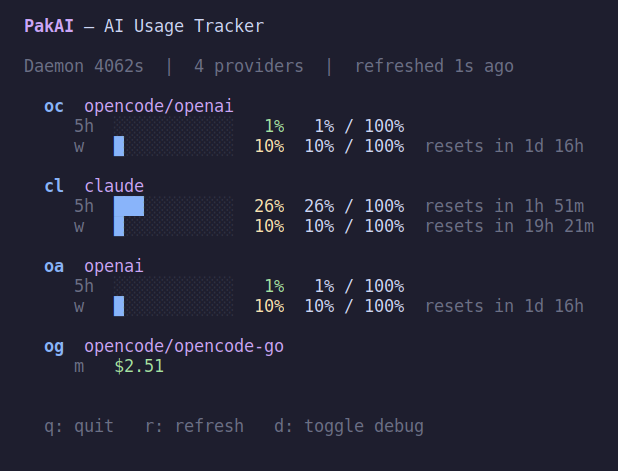
\includegraphics[width=0.58\linewidth]{pakai-dashboard}

\vspace{1.5cm}

% Tool name — the main title
{\fontsize{58}{66}\selectfont\bfseries\sffamily\color{termfg} PakAI\par}

\vspace{0.5cm}

% Tagline: casual, not formal
{\large\color{termsubtext} pantau semua AI-mu, dari terminal\par}

\vfill

% Supported providers — breaks the gap and shows scope at a glance
{\small\ttfamily\color{termsubtext}
  claude \enspace\textbullet\enspace codex \enspace\textbullet\enspace opencode
\par}

\vspace{0.3cm}

{\footnotesize\color{termsurface}
  multi-provider \enspace\textbullet\enspace
  real-time \enspace\textbullet\enspace
  open source
\par}

\vspace{1.4cm}

% Thin separator
{\color{termsurface}\rule{0.40\linewidth}{0.4pt}\par}

\vspace{0.6cm}

% Authors — informal bullet list on two lines
{\small\color{termsubtext}
  Dian Hanifudin Subhi \enspace\textbullet\enspace Dhebys Suryani Hormansyah \\[0.25em]
  Agung Nugroho Pramudhita \enspace\textbullet\enspace Sofyan Noor Arief\par
}

\vspace{0.4cm}

{\footnotesize\color{termsubtext} v1.0 \enspace\textbullet\enspace Mei 2026\par}

\vspace*{1.8cm}

\end{titlepage}
\restoregeometry
\pagecolor{white}
\color{black}

% ─── Colophon ────────────────────────────────────────────────────────────────
\thispagestyle{empty}
\vspace*{\fill}
\begin{center}
  \small
  PakAI adalah alat bantu pemantau penggunaan langganan AI yang bersifat \\
  open-source dan gratis digunakan.\\[1em]
  \url{https://github.com/dhanifudin/pakai}
\end{center}
\vspace*{\fill}

\tableofcontents
\clearpage

\mainmatter

\chapter{Pendahuluan}

\section{Apa itu PakAI?}

\textbf{PakAI} (dijalankan dengan perintah \cmd{pakai}) adalah alat bantu berbasis terminal
untuk memantau penggunaan langganan layanan AI secara terpadu. Alat ini menampilkan
sisa kuota dan biaya untuk beberapa penyedia AI sekaligus dalam satu tampilan yang
ringkas.

PakAI mendukung tiga penyedia layanan AI:

\begin{itemize}
  \item \textbf{Claude} (Anthropic): memantau persentase penggunaan pesan per 5 jam,
        mingguan, dan bulanan melalui OAuth API.
  \item \textbf{OpenAI Codex}: memantau kuota penggunaan per 5 jam dan mingguan
        melalui OAuth API.
  \item \textbf{OpenCode Go}: memantau biaya penggunaan per penyedia dari
        database lokal SQLite.
\end{itemize}

\section{Fitur Utama}

\begin{itemize}
  \item Pemantauan multi-penyedia dalam satu perintah.
  \item Tiga jendela waktu: 5 jam, mingguan, dan bulanan.
  \item Tampilan berwarna: hijau (aman), kuning (peringatan), merah (kritis).
  \item Empat mode tampilan: status CLI, tmux, Waybar, dan dashboard TUI.
  \item Daemon latar belakang dengan pembaruan otomatis dan API HTTP.
  \item Pengaturan melalui berkas konfigurasi TOML.
  \item Deteksi otomatis penyedia yang terinstal.
\end{itemize}

\section{Tampilan Aplikasi}

Gambar di bawah menampilkan output perintah \cmd{pakai status} yang menunjukkan
ringkasan penggunaan semua penyedia yang terdeteksi.

\begin{figure}[h]
  \centering
  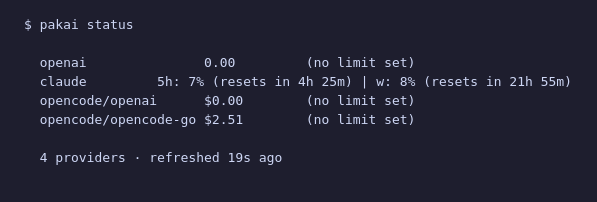
\includegraphics[width=0.85\linewidth]{pakai-status}
  \caption{Output \texttt{pakai status}: ringkasan penggunaan semua penyedia}
\end{figure}

\section{Cara Kerja}

PakAI berjalan sebagai \textit{background daemon} yang secara berkala mengambil data
penggunaan dari setiap penyedia. Data ini kemudian ditampilkan melalui berbagai
antarmuka:

\begin{enumerate}
  \item \textbf{Daemon} berjalan di port 7731 dan menyimpan data terbaru.
  \item Perintah \cmd{pakai status}, \cmd{pakai tmux}, dan \cmd{pakai waybar}
        mengambil data dari daemon melalui HTTP.
  \item \cmd{pakai dashboard} menampilkan antarmuka TUI interaktif dengan
        pembaruan langsung (\textit{live update}).
\end{enumerate}

\chapter{Persyaratan Sistem}

\section{Sistem Operasi}

PakAI dirancang untuk berjalan di lingkungan Unix dan Unix-like. Sistem yang didukung:

\begin{itemize}
  \item \textbf{Linux} (Ubuntu, Debian, Fedora, Arch, NixOS, dan distribusi lainnya)
  \item \textbf{macOS} (Ventura, Sonoma, Sequoia, dan versi lebih baru)
  \item \textbf{WSL2} (Windows Subsystem for Linux 2) di Windows 10/11
\end{itemize}

\section{Perangkat Lunak yang Dibutuhkan}

\subsection{Go (untuk build dari kode sumber)}

Diperlukan Go versi \textbf{1.21 atau lebih baru} jika ingin melakukan kompilasi
sendiri dari kode sumber.

\begin{lstlisting}[style=terminal]
$ go version
go version go1.25.0 linux/amd64
\end{lstlisting}

Unduh Go dari \url{https://go.dev/dl/} atau gunakan manajer versi seperti
\textbf{asdf}, \textbf{mise}, atau \textbf{nix}.

\subsection{Penyedia AI (opsional, sesuai kebutuhan)}

Pasang dan autentikasi penyedia yang ingin dipantau:

\begin{center}
\begin{tabular}{lll}
\toprule
\textbf{Penyedia} & \textbf{Perangkat} & \textbf{Autentikasi} \\
\midrule
Claude & Claude Code CLI & \cmd{claude login} \\
OpenAI Codex & Pi atau Codex CLI & Login di sumber yang dipilih \\
OpenCode Go & OpenCode & Langganan di opencode.ai \\
\bottomrule
\end{tabular}
\end{center}

Tidak perlu memasang semua penyedia. PakAI akan mendeteksi otomatis penyedia
mana yang tersedia.

\section{Persyaratan Jaringan}

Semua penyedia yang didukung memerlukan koneksi internet:

\begin{itemize}
  \item \textbf{Claude} dan \textbf{OpenAI Codex} memerlukan koneksi internet untuk
        mengambil data penggunaan melalui API OAuth.
  \item \textbf{OpenCode Go} memerlukan koneksi internet untuk menjalankan sesi
        OpenCode CLI. PakAI sendiri membaca data penggunaan dari database lokal
        yang dibuat oleh OpenCode, tetapi OpenCode CLI membutuhkan jaringan saat
        digunakan.
\end{itemize}

\chapter{Instalasi}

\section{Metode 1: Install dari Go (Direkomendasikan)}

Cara termudah adalah menggunakan \cmd{go install} untuk mengunduh dan mengkompilasi
PakAI secara langsung:

\begin{lstlisting}[style=terminal]
$ go install github.com/dhanifudin/pakai/cmd/pakai@latest
\end{lstlisting}

Pastikan direktori \texttt{\$GOPATH/bin} (biasanya \texttt{\textasciitilde/go/bin})
sudah ada di \texttt{\$PATH}:

\begin{lstlisting}[style=terminal]
# Tambahkan ke ~/.bashrc atau ~/.zshrc
export PATH="$PATH:$HOME/go/bin"
\end{lstlisting}

\section{Metode 2: Build dari Kode Sumber}

\subsection{Kloning repositori}

\begin{lstlisting}[style=terminal]
$ git clone https://github.com/dhanifudin/pakai.git
$ cd pakai
\end{lstlisting}

\subsection{Kompilasi}

\begin{lstlisting}[style=terminal]
$ go build -ldflags="-s -w" -o pakai ./cmd/pakai
\end{lstlisting}

Atau gunakan Makefile yang sudah disediakan:

\begin{lstlisting}[style=terminal]
$ make build
\end{lstlisting}

\subsection{Pasang ke PATH}

\begin{lstlisting}[style=terminal]
$ sudo mv pakai /usr/local/bin/
# atau ke direktori lokal tanpa sudo:
$ mv pakai ~/.local/bin/
\end{lstlisting}

\section{Metode 3: Binary Release}

Binary siap pakai tersedia di halaman \textit{Releases} GitHub untuk arsitektur
Linux AMD64 dan ARM64:

\begin{enumerate}
  \item Kunjungi \url{https://github.com/dhanifudin/pakai/releases}
  \item Unduh arsip yang sesuai, misalnya:\\
        \texttt{pakai\_1.0.0\_linux\_amd64.tar.gz}
  \item Ekstrak dan pindahkan binary:
\end{enumerate}

\begin{lstlisting}[style=terminal]
$ tar -xzf pakai_1.0.0_linux_amd64.tar.gz
$ chmod +x pakai
$ mv pakai ~/.local/bin/
\end{lstlisting}

\section{Verifikasi Instalasi}

Setelah instalasi, mulai daemon lalu jalankan perintah status untuk memverifikasi
PakAI berjalan dengan benar:

\begin{lstlisting}[style=terminal]
$ pakai daemon start
$ pakai status
\end{lstlisting}

\begin{figure}[h]
  \centering
  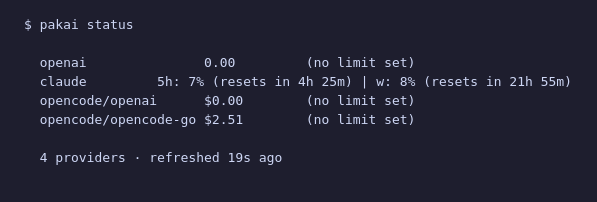
\includegraphics[width=0.85\linewidth]{pakai-status}
  \caption{Output \texttt{pakai status} setelah instalasi berhasil}
\end{figure}

Jika perintah tidak ditemukan, pastikan direktori instalasi ada di \texttt{\$PATH}.

\begin{warningbox}
  Jika menggunakan \textbf{asdf} atau \textbf{mise} sebagai manajer versi Go,
  pastikan shim untuk \texttt{pakai} sudah diperbarui setelah instalasi.
  Jalankan \cmd{asdf reshim golang} atau \cmd{mise reshim} setelah proses instalasi.
\end{warningbox}

\chapter{Konfigurasi Awal}

\section{Perintah Setup Otomatis}

PakAI menyediakan perintah \cmd{pakai setup} yang mendeteksi penyedia yang terinstal,
menulis unit systemd, dan menampilkan cuplikan konfigurasi yang siap digunakan.

\begin{lstlisting}[style=terminal]
$ pakai setup
\end{lstlisting}

\begin{figure}[h]
  \centering
  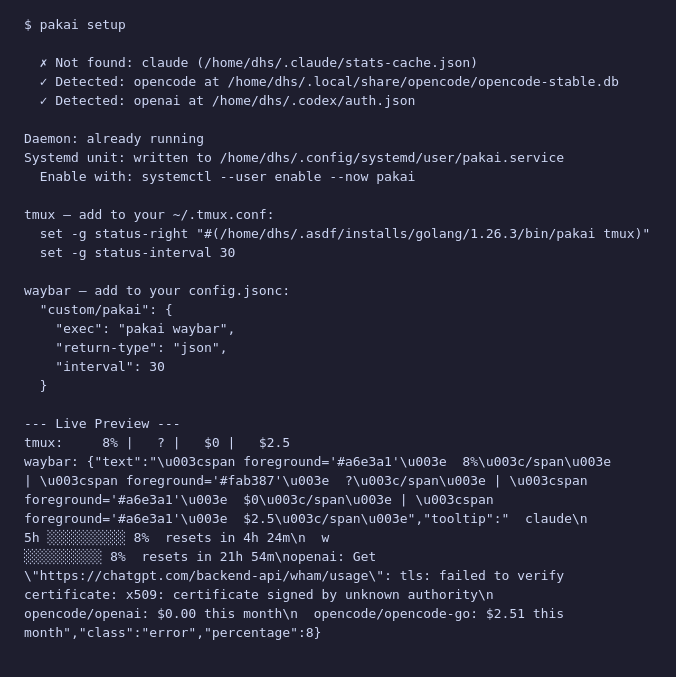
\includegraphics[width=0.88\linewidth]{pakai-setup}
  \caption{Output \texttt{pakai setup}: deteksi penyedia dan konfigurasi otomatis}
\end{figure}

\subsection{Yang Dilakukan oleh \texttt{pakai setup}}

\begin{enumerate}
  \item \textbf{Deteksi penyedia}: memeriksa jalur berikut:
    \begin{itemize}
      \item Claude: \texttt{\textasciitilde/.claude/stats-cache.json}
      \item OpenCode Go: \texttt{\textasciitilde/.local/share/opencode/opencode-stable.db}
            atau \texttt{opencode.db}
      \item OpenAI Codex: \texttt{\textasciitilde/.codex/auth.json}
    \end{itemize}
  \item \textbf{Memulai daemon} jika belum berjalan.
  \item \textbf{Membuat unit systemd} di\\
        \texttt{\textasciitilde/.config/systemd/user/pakai.service}.
  \item \textbf{Menampilkan cuplikan konfigurasi} untuk tmux dan Waybar.
\end{enumerate}

\section{Memulai Daemon}

Daemon adalah proses latar belakang yang mengambil dan menyimpan data penggunaan.
Tanpa daemon, perintah-perintah PakAI tidak akan menampilkan data.

\subsection{Memulai daemon secara manual}

\begin{lstlisting}[style=terminal]
$ pakai daemon start
Daemon started (port 7731)
\end{lstlisting}

\subsection{Memeriksa status daemon}

\begin{lstlisting}[style=terminal]
$ pakai daemon status
\end{lstlisting}

\begin{figure}[h]
  \centering
  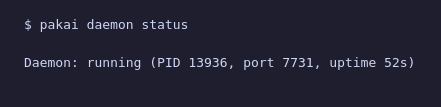
\includegraphics[width=0.72\linewidth]{pakai-daemon-status}
  \caption{Output \texttt{pakai daemon status}}
\end{figure}

\subsection{Menghentikan daemon}

\begin{lstlisting}[style=terminal]
$ pakai daemon stop
\end{lstlisting}

\section{Konfigurasi Autostart dengan Systemd}

Agar daemon berjalan otomatis saat login, aktifkan unit systemd yang dibuat oleh
\cmd{pakai setup}:

\begin{lstlisting}[style=terminal]
$ systemctl --user enable --now pakai
$ systemctl --user status pakai
\end{lstlisting}

Isi unit systemd yang dibuat secara otomatis:

\begin{lstlisting}[style=toml]
[Unit]
Description=PakAI usage tracker daemon
After=default.target

[Service]
ExecStart=/home/user/.local/bin/pakai daemon start --foreground
Restart=on-failure
RestartSec=5

[Install]
WantedBy=default.target
\end{lstlisting}

\begin{tipbox}
  Gunakan \cmd{journalctl --user -u pakai -f} untuk melihat log daemon secara
  langsung (\textit{real-time}).
\end{tipbox}

\section{Autentikasi Penyedia}

\subsection{Claude}

Claude menggunakan OAuth yang dikelola oleh Claude Code CLI. Jalankan:

\begin{lstlisting}[style=terminal]
$ claude login
\end{lstlisting}

Kredensial disimpan di \texttt{\textasciitilde/.claude/.credentials.json}.

\subsection{OpenAI Codex}

\begin{lstlisting}[style=terminal]
$ codex login
\end{lstlisting}

Kredensial disimpan di \texttt{\textasciitilde/.codex/auth.json}.

\subsection{OpenCode Go}

OpenCode Go tidak memerlukan login tambahan. PakAI membaca langsung dari database
SQLite yang dibuat oleh OpenCode. Pastikan OpenCode sudah pernah digunakan minimal
satu kali sehingga database terbentuk di:

\begin{lstlisting}[style=terminal]
~/.local/share/opencode/opencode-stable.db
\end{lstlisting}

\chapter{Penggunaan Dasar}

\section{Mengapa Memantau Penggunaan AI?}

Berlangganan lebih dari satu layanan AI berarti mengelola beberapa jendela waktu
kuota yang berbeda: Claude membatasi pesan per 5 jam dan mingguan, OpenAI Codex
membatasi per 5 jam dan mingguan, sementara OpenCode mencatat biaya token secara
langsung. Tanpa pemantauan, ada tiga masalah yang sering dialami:

\begin{itemize}
  \item \textbf{Kuota habis di tengah pekerjaan.} Claude atau Codex berhenti
        merespons tanpa peringatan sebelumnya, memutus alur kerja saat sedang
        fokus.
  \item \textbf{Biaya tak terduga.} Token yang digunakan melalui OpenCode
        langsung ditagih; tanpa visibilitas, tagihan bulanan bisa mengejutkan.
  \item \textbf{Konteks berpindah-pindah.} Memeriksa kuota berarti membuka
        dasbor web masing-masing penyedia, memecah konsentrasi dari terminal.
\end{itemize}

PakAI menyelesaikan ketiga masalah ini dengan satu perintah di terminal. Status
semua penyedia tersedia setiap saat — di status bar tmux, di panel Waybar, maupun
di dashboard TUI layar penuh — tanpa harus meninggalkan lingkungan kerja.

\begin{tipbox}
  PakAI cocok untuk siapa saja yang menggunakan dua atau lebih layanan AI
  berbayar dan ingin tahu kapan harus beralih penyedia atau mengistirahatkan sesi
  agar kuota tidak terbuang.
\end{tipbox}

\section{Memeriksa Status Penggunaan}

Perintah utama untuk melihat ringkasan penggunaan semua penyedia:

\begin{lstlisting}[style=terminal]
$ pakai status
\end{lstlisting}

\begin{figure}[h]
  \centering
  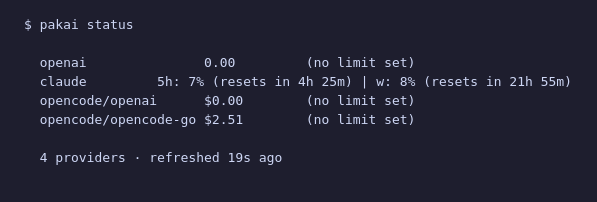
\includegraphics[width=0.85\linewidth]{pakai-status}
  \caption{Output \texttt{pakai status}: ringkasan semua penyedia aktif}
\end{figure}

Output menampilkan:
\begin{itemize}
  \item Nama penyedia dan label yang dikonfigurasi.
  \item Persentase atau biaya penggunaan per jendela waktu (5j, mingguan, bulanan).
  \item Waktu reset atau sisa waktu jendela.
  \item Jumlah penyedia aktif dan waktu pembaruan terakhir.
\end{itemize}

\subsection{Output JSON}

Tambahkan flag \cmd{--json} untuk mendapatkan output dalam format JSON mentah:

\begin{lstlisting}[style=terminal]
$ pakai status --json
\end{lstlisting}

\section{Dashboard TUI Interaktif}

Dashboard TUI menampilkan tampilan penuh layar dengan pembaruan langsung:

\begin{lstlisting}[style=terminal]
$ pakai dashboard
\end{lstlisting}

\begin{figure}[ht]
  \centering
  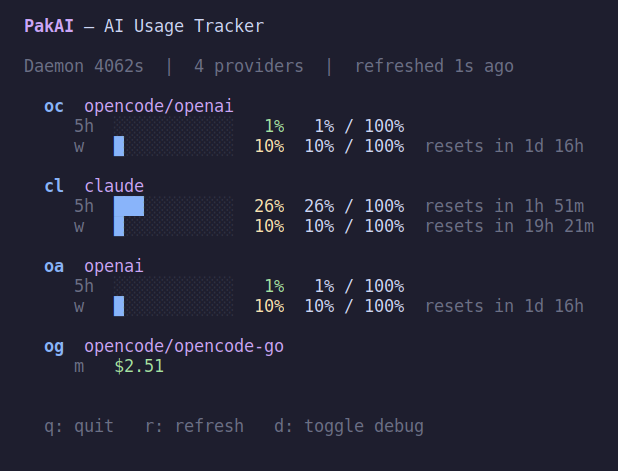
\includegraphics[width=0.90\linewidth]{pakai-dashboard}
  \caption{Dashboard TUI PakAI: empat penyedia aktif dengan progress bar
           dan sisa waktu reset per jendela waktu}
\end{figure}

Dashboard diperbarui secara otomatis setiap kali daemon menerima data baru dari
penyedia. Tampilan dibagi per penyedia, masing-masing menampilkan baris untuk
setiap jendela waktu yang aktif.

\subsection{Membaca tampilan dashboard}

Setiap baris di dalam dashboard mengikuti format berikut:

\begin{center}
\begin{tabular}{lp{10cm}}
\toprule
\textbf{Kolom} & \textbf{Keterangan} \\
\midrule
Ikon / kode & Ikon Nerd Font penyedia; fallback dua huruf bila font tidak tersedia. \\[4pt]
Nama penyedia & Label penyedia, termasuk sub-penyedia OpenCode. \\[4pt]
Jendela waktu & \texttt{5h} (5 jam), \texttt{w} (mingguan), \texttt{m} (bulanan). \\[4pt]
Progress bar & Bar 12 segmen menunjukkan proporsi penggunaan saat ini. \\[4pt]
Persentase & Angka persentase atau biaya dalam dolar (\texttt{\$}). \\[4pt]
Waktu reset & Sisa waktu sebelum kuota jendela direset. \\
\bottomrule
\end{tabular}
\end{center}

\subsection{Kode warna}

PakAI menggunakan tiga warna untuk persentase penggunaan:

\begin{itemize}
  \item \textbf{Hijau} — penggunaan di bawah ambang peringatan (aman).
  \item \textbf{Kuning} — mendekati batas; pertimbangkan untuk beralih penyedia
        atau mengurangi frekuensi permintaan.
  \item \textbf{Merah} — mendekati atau melebihi batas; kuota hampir habis.
\end{itemize}

Ambang kuning dan merah dapat dikonfigurasi melalui \cmd{pakai config set}
(lihat Bab~\ref{ch:konfigurasi-lanjutan}).

\subsection{Kapan dashboard berguna}

Dashboard layar penuh paling berguna dalam skenario berikut:

\begin{itemize}
  \item \textbf{Sebelum sesi panjang}: periksa penyedia mana yang masih punya
        kuota cukup sebelum memulai pekerjaan berat.
  \item \textbf{Saat jendela waktu hampir reset}: pantau kolom \textit{resets in}
        untuk memilih waktu terbaik memulai ulang sesi.
  \item \textbf{Membandingkan biaya}: lihat akumulasi biaya dolar OpenCode
        berdampingan dengan kuota pesan Claude dan Codex.
  \item \textbf{Debugging penyedia}: tekan \texttt{d} untuk melihat JSON mentah
        yang dikirim setiap penyedia, berguna saat ada anomali data.
\end{itemize}

\textbf{Tombol keyboard:}
\begin{center}
\begin{tabular}{ll}
\toprule
\textbf{Tombol} & \textbf{Fungsi} \\
\midrule
\texttt{q} & Keluar dari dashboard \\
\texttt{r} & Muat ulang data secara manual \\
\texttt{d} & Aktifkan/nonaktifkan mode debug (tampilkan JSON mentah) \\
\bottomrule
\end{tabular}
\end{center}

\begin{infobox}
  Jika daemon belum berjalan, jalankan \cmd{pakai daemon start} terlebih dahulu
  sebelum membuka dashboard.
\end{infobox}

\section{Output untuk Tmux}

Perintah \cmd{pakai tmux} menghasilkan string ringkas untuk status bar tmux:

\begin{lstlisting}[style=terminal]
$ pakai tmux
  7% |  8% |  $0.00
\end{lstlisting}

Output menggunakan ikon Nerd Font untuk setiap penyedia. Pastikan terminal
menggunakan font yang mendukung Nerd Font.

\section{Output untuk Waybar}

Perintah \cmd{pakai waybar} menghasilkan JSON untuk modul kustom Waybar:

\begin{lstlisting}[style=terminal]
$ pakai waybar
\end{lstlisting}

\begin{figure}[h]
  \centering
  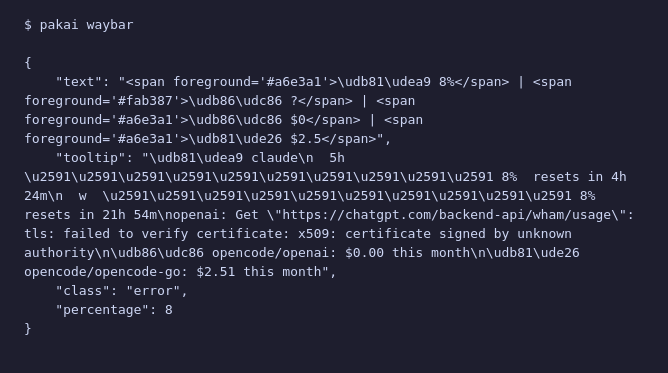
\includegraphics[width=0.85\linewidth]{pakai-waybar}
  \caption{Output JSON dari \texttt{pakai waybar}}
\end{figure}

Format output JSON:
\begin{lstlisting}[style=toml]
{
  "text": "<teks tampilan>",
  "tooltip": "<detail per penyedia>",
  "class": "ok|warning|critical|error",
  "percentage": 0
}
\end{lstlisting}

\section{Men-debug Penyedia}

Untuk memeriksa detail data satu penyedia tertentu:

\begin{lstlisting}[style=terminal]
$ pakai provider debug claude
$ pakai provider debug opencode
$ pakai provider debug openai
\end{lstlisting}

\begin{figure}[h]
  \centering
  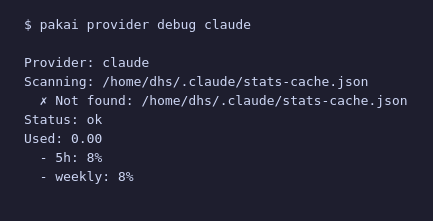
\includegraphics[width=0.75\linewidth]{pakai-provider-debug}
  \caption{Output \texttt{pakai provider debug claude}}
\end{figure}

\section{Completion Shell}

Aktifkan pelengkapan otomatis perintah (tab completion) untuk shell Anda:

\begin{lstlisting}[style=terminal]
# Bash
$ pakai completion bash >> ~/.bashrc

# Zsh
$ pakai completion zsh >> ~/.zshrc

# Fish
$ pakai completion fish > ~/.config/fish/completions/pakai.fish
\end{lstlisting}

\chapter{Integrasi}

\section{Integrasi Tmux}

\subsection{Konfigurasi dasar}

Tambahkan baris berikut ke berkas \texttt{\textasciitilde/.tmux.conf}:

\begin{lstlisting}[style=toml]
# Tampilkan status PakAI di status bar kanan
set -g status-right "#(pakai tmux)"
set -g status-interval 30

# Opsional: perpanjang lebar status bar
set -g status-right-length 100
\end{lstlisting}

Muat ulang konfigurasi tmux tanpa harus me-restart:

\begin{lstlisting}[style=terminal]
$ tmux source-file ~/.tmux.conf
\end{lstlisting}

\subsection{Konfigurasi dengan tmux-powerline}

\begin{sloppypar}
Jika menggunakan \textit{tmux-powerline} atau tema kustom, sesuaikan
\texttt{status-right} dengan format yang digunakan tema Anda.
\end{sloppypar}

\begin{tipbox}
  Jalankan \cmd{pakai setup tmux} untuk mendapatkan cuplikan konfigurasi tmux
  yang siap tempel (\textit{ready-to-paste}).
\end{tipbox}

\subsection{Persyaratan font}

Ikon penyedia menggunakan karakter \textbf{Nerd Font}. Pastikan terminal dan tmux
menggunakan font Nerd Font seperti:
\begin{itemize}
  \item JetBrains Mono Nerd Font
  \item Fira Code Nerd Font
  \item DejaVu Sans Mono Nerd Font
\end{itemize}

Jika ikon tidak muncul, ikon akan digantikan dengan dua huruf pertama nama
penyedia (misalnya \texttt{cl} untuk Claude).

\section{Integrasi Waybar}

\subsection{Konfigurasi modul}

Tambahkan modul kustom ke berkas konfigurasi Waybar (biasanya
\path{~/.config/waybar/config.jsonc}):

\begin{lstlisting}[style=toml]
"custom/pakai": {
    "exec": "pakai waybar",
    "return-type": "json",
    "interval": 30,
    "tooltip": true,
    "format": "{}",
    "on-click": "pakai dashboard"
}
\end{lstlisting}

\begin{sloppypar}
Tambahkan \texttt{"custom/pakai"} ke array \texttt{modules-right} (atau
\texttt{modules-left}/\texttt{modules-center} sesuai preferensi):
\end{sloppypar}

\begin{lstlisting}[style=toml]
"modules-right": [
    "custom/pakai",
    "clock",
    "battery"
]
\end{lstlisting}

\subsection{Konfigurasi CSS}

Tambahkan style ke berkas CSS Waybar (\texttt{style.css}) untuk
pewarnaan berdasarkan status:

\begin{lstlisting}[style=toml]
#custom-pakai {
    padding: 0 8px;
    color: #cdd6f4;
}

#custom-pakai.ok {
    color: #a6e3a1;
}

#custom-pakai.warning {
    color: #f9e2af;
}

#custom-pakai.critical {
    color: #f38ba8;
}

#custom-pakai.error {
    color: #fab387;
}
\end{lstlisting}

\subsection{Tooltip}

\begin{sloppypar}
Waybar menampilkan tooltip berisi rincian penggunaan per jendela waktu ketika
kursor diarahkan ke modul PakAI. Pastikan \texttt{"tooltip": true} sudah
dikonfigurasi di modul.
\end{sloppypar}

\begin{tipbox}
  Jalankan \cmd{pakai setup waybar} untuk mendapatkan cuplikan konfigurasi
  Waybar yang lengkap, termasuk JSON modul dan CSS.
\end{tipbox}

\section{Integrasi Shell Prompt}

PakAI juga dapat ditampilkan di prompt shell. Contoh untuk Zsh dengan
\textbf{Starship}:

\begin{lstlisting}[style=toml]
# ~/.config/starship.toml
[custom.pakai]
command = "pakai tmux"
when = "pakai daemon status"
format = "[$output]($style) "
style = "green"
\end{lstlisting}

\chapter{Konfigurasi Lanjutan}
\label{ch:konfigurasi-lanjutan}

\section{Berkas Konfigurasi}

PakAI menyimpan konfigurasi di:
\begin{itemize}
  \item \texttt{\$XDG\_CONFIG\_HOME/pakai/config.toml}: jika variabel tersebut diset.
  \item \texttt{\textasciitilde/.config/pakai/config.toml}: lokasi default.
\end{itemize}

Berkas dibuat secara otomatis saat pertama kali menyimpan konfigurasi.

\section{Melihat Semua Konfigurasi}

\begin{lstlisting}[style=terminal]
$ pakai config list
\end{lstlisting}

\begin{figure}[h]
  \centering
  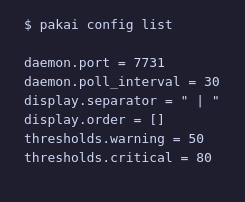
\includegraphics[width=0.6\linewidth]{pakai-config-list}
  \caption{Output \texttt{pakai config list}: semua konfigurasi aktif}
\end{figure}

\section{Mengubah Konfigurasi}

Gunakan \cmd{pakai config set \textit{kunci} \textit{nilai}} untuk mengubah nilai:

\begin{lstlisting}[style=terminal]
$ pakai config set daemon.port 7732
$ pakai config get daemon.port
\end{lstlisting}

\section{Referensi Kunci Konfigurasi}

\subsection{Konfigurasi Daemon}

\begin{center}
\begin{tabular}{lllp{5cm}}
\toprule
\textbf{Kunci} & \textbf{Tipe} & \textbf{Default} & \textbf{Keterangan} \\
\midrule
\texttt{daemon.port} & integer & 7731 & Port HTTP daemon (1--65535) \\
\texttt{daemon.poll\_interval} & integer & 30 & Interval polling dalam detik ($\geq 1$) \\
\bottomrule
\end{tabular}
\end{center}

\begin{lstlisting}[style=terminal]
$ pakai config set daemon.poll_interval 15
$ pakai config set daemon.port 7732
\end{lstlisting}

\subsection{Konfigurasi Tampilan}

\begin{center}
\begin{tabular}{lllp{5cm}}
\toprule
\textbf{Kunci} & \textbf{Tipe} & \textbf{Default} & \textbf{Keterangan} \\
\midrule
\texttt{display.separator} & string & \texttt{ | } & Pemisah antar penyedia \\
\texttt{display.order} & string & (auto) & Urutan penyedia, dipisah koma \\
\bottomrule
\end{tabular}
\end{center}

\begin{lstlisting}[style=terminal]
$ pakai config set display.separator " - "
$ pakai config set display.order "claude,opencode,openai"
\end{lstlisting}

\subsection{Konfigurasi Ambang Batas}

\begin{center}
\begin{tabular}{lllp{5cm}}
\toprule
\textbf{Kunci} & \textbf{Tipe} & \textbf{Default} & \textbf{Keterangan} \\
\midrule
\texttt{thresholds.warning} & integer & 50 & Ambang peringatan (0--100\%) \\
\texttt{thresholds.critical} & integer & 80 & Ambang kritis (0--100\%) \\
\bottomrule
\end{tabular}
\end{center}

\begin{lstlisting}[style=terminal]
$ pakai config set thresholds.warning 60
$ pakai config set thresholds.critical 85
\end{lstlisting}

\subsection{Konfigurasi Per Penyedia}

Setiap penyedia dapat dikonfigurasi dengan format \texttt{provider.\textit{id}.\textit{kunci}}:

\begin{center}
\begin{tabular}{lllp{4.5cm}}
\toprule
\textbf{Kunci} & \textbf{Tipe} & \textbf{Default} & \textbf{Keterangan} \\
\midrule
\texttt{provider.\textit{id}.enabled} & bool & true & Aktifkan/nonaktifkan penyedia \\
\texttt{provider.\textit{id}.label} & string & (id) & Label tampilan kustom \\
\texttt{provider.\textit{id}.limit} & float & 0 & Batas biaya dalam USD ($\geq 0$) \\
\bottomrule
\end{tabular}
\end{center}

ID penyedia yang tersedia: \texttt{claude}, \texttt{opencode}, \texttt{openai},
\texttt{opencode/openai}, \texttt{opencode/opencode-go}.

\begin{lstlisting}[style=terminal]
# Atur label kustom untuk Claude
$ pakai config set provider.claude.label "Klaude"

# Atur batas bulanan untuk OpenCode Go
$ pakai config set provider.opencode-go.limit 60

# Nonaktifkan penyedia OpenAI sementara
$ pakai config set provider.openai.enabled false
\end{lstlisting}

\section{Contoh Berkas Konfigurasi Lengkap}

\begin{lstlisting}[style=toml]
[daemon]
port = 7731
poll_interval = 30

[display]
separator = " | "
order = "claude,opencode/opencode-go,openai"

[thresholds]
warning = 50
critical = 80

[provider.claude]
enabled = true
label = "Claude"

[provider.openai]
enabled = true
label = "Codex"

[provider.opencode]
enabled = true
label = "OpenCode"

[provider."opencode/opencode-go"]
enabled = true
limit = 60.0
\end{lstlisting}

\section{Mock Provider (untuk Pengujian)}

PakAI mendukung penyedia palsu (\textit{mock}) untuk keperluan pengujian tampilan:

\begin{lstlisting}[style=terminal]
# Buat mock dengan 75% penggunaan
$ pakai provider mock test-ai --used 75 --limit 100 --unit messages

# Hapus mock
$ pakai provider unmock test-ai
\end{lstlisting}

\chapter{Referensi Perintah}

Berikut adalah daftar lengkap semua perintah yang tersedia di PakAI.

\section{Perintah Utama}

\begin{longtable}{p{6.5cm}p{8cm}}
\toprule
\textbf{Perintah} & \textbf{Keterangan} \\
\midrule
\endhead
\cmd{pakai version} & Menampilkan versi PakAI yang terinstal. \\[4pt]
\cmd{pakai status} & Menampilkan ringkasan penggunaan semua penyedia. \\[4pt]
\cmd{pakai status --json} & Menampilkan data penggunaan dalam format JSON mentah. \\[4pt]
\cmd{pakai tmux} & Menghasilkan string ringkas untuk status bar tmux. \\[4pt]
\cmd{pakai waybar} & Menghasilkan JSON untuk modul kustom Waybar. \\[4pt]
\cmd{pakai dashboard} & Membuka antarmuka TUI interaktif dengan pembaruan langsung. \\[4pt]
\cmd{pakai completion \textit{shell}} & Menghasilkan skrip \textit{tab completion} (\texttt{bash}/\texttt{zsh}/\texttt{fish}). \\
\bottomrule
\end{longtable}

\section{Perintah Daemon}

\begin{longtable}{p{6.5cm}p{8cm}}
\toprule
\textbf{Perintah} & \textbf{Keterangan} \\
\midrule
\endhead
\cmd{pakai daemon start} & Menjalankan daemon di latar belakang. \\[4pt]
\cmd{pakai daemon start --foreground} & Menjalankan daemon di latar depan (untuk systemd). \\[4pt]
\cmd{pakai daemon stop} & Menghentikan daemon yang berjalan. \\[4pt]
\cmd{pakai daemon status} & Menampilkan status daemon (PID, port, uptime). \\
\bottomrule
\end{longtable}

\section{Perintah Setup}

\begin{longtable}{p{6.5cm}p{8cm}}
\toprule
\textbf{Perintah} & \textbf{Keterangan} \\
\midrule
\endhead
\cmd{pakai setup} & Deteksi penyedia, buat unit systemd, tampilkan konfigurasi. \\[4pt]
\cmd{pakai setup tmux} & Tampilkan cuplikan konfigurasi tmux. \\[4pt]
\cmd{pakai setup waybar} & Tampilkan cuplikan konfigurasi Waybar dan CSS. \\
\bottomrule
\end{longtable}

\section{Perintah Konfigurasi}

\begin{longtable}{p{6.5cm}p{8cm}}
\toprule
\textbf{Perintah} & \textbf{Keterangan} \\
\midrule
\endhead
\cmd{pakai config list} & Menampilkan semua konfigurasi aktif. \\[4pt]
\cmd{pakai config get \textit{kunci}} & Menampilkan nilai satu kunci konfigurasi. \\[4pt]
\cmd{pakai config set \textit{kunci} \textit{nilai}} & Mengatur nilai kunci konfigurasi. \\
\bottomrule
\end{longtable}

\section{Perintah Penyedia}

\begin{longtable}{p{6.5cm}p{8cm}}
\toprule
\textbf{Perintah} & \textbf{Keterangan} \\
\midrule
\endhead
\cmd{pakai provider debug \textit{id}} & Menampilkan data debug untuk penyedia tertentu. \\[4pt]
\cmd{pakai provider mock \textit{id}} & Membuat penyedia palsu untuk pengujian. \\[4pt]
\quad \texttt{--used \textit{float}} & Nilai penggunaan (default: 0). \\[2pt]
\quad \texttt{--limit \textit{float}} & Nilai batas, 0 = tanpa batas (default: 0). \\[2pt]
\quad \texttt{--unit \textit{string}} & Satuan: \texttt{messages}, \texttt{tokens}, atau \texttt{usd}. \\[4pt]
\cmd{pakai provider unmock \textit{id}} & Menghapus penyedia palsu. \\
\bottomrule
\end{longtable}

\section{HTTP API Daemon}

Daemon mengekspos API HTTP lokal di \texttt{http://127.0.0.1:7731}.

\begin{longtable}{llp{7cm}}
\toprule
\textbf{Method} & \textbf{Endpoint} & \textbf{Keterangan} \\
\midrule
\endhead
GET & \texttt{/health} & Status daemon, uptime, jumlah koneksi. \\[4pt]
GET & \texttt{/status} & Data penggunaan semua penyedia (JSON). \\[4pt]
GET & \texttt{/events} & \textit{Server-Sent Events} untuk pembaruan langsung. \\[4pt]
PUT & \texttt{/mock/\textit{name}} & Memasukkan data mock penyedia. \\[4pt]
DELETE & \texttt{/mock/\textit{name}} & Menghapus data mock penyedia. \\[4pt]
GET & \texttt{/debug/\textit{name}} & Debug data satu penyedia. \\
\bottomrule
\end{longtable}

\begin{lstlisting}[style=terminal]
# Contoh mengakses API langsung
$ curl -s http://127.0.0.1:7731/health | python3 -m json.tool
$ curl -s http://127.0.0.1:7731/status | python3 -m json.tool
\end{lstlisting}

\chapter{Pemecahan Masalah}

\section{Masalah Instalasi}

\subsection{Perintah \texttt{pakai} tidak ditemukan}

\textbf{Gejala:} \texttt{bash: pakai: command not found}

\textbf{Penyebab:} Direktori instalasi tidak ada di \texttt{\$PATH}.

\textbf{Solusi:}
\begin{lstlisting}[style=terminal]
# Cari lokasi binary
$ which pakai || find ~/go ~/go/bin ~/.local/bin -name pakai 2>/dev/null

# Tambahkan ke PATH (sesuaikan path yang ditemukan)
$ echo 'export PATH="$PATH:$HOME/go/bin"' >> ~/.bashrc
$ source ~/.bashrc
\end{lstlisting}

Jika menggunakan \textbf{asdf}:
\begin{lstlisting}[style=terminal]
$ asdf reshim golang
\end{lstlisting}

\subsection{Build gagal: versi Go terlalu lama}

\textbf{Gejala:} \texttt{requires go >= 1.21}

\textbf{Solusi:} Perbarui Go ke versi 1.21 atau lebih baru.
\begin{lstlisting}[style=terminal]
$ go version        # cek versi saat ini
$ asdf install golang latest   # update via asdf
\end{lstlisting}

\section{Masalah Daemon}

\subsection{Daemon gagal dimulai: port sudah digunakan}

\textbf{Gejala:} \texttt{port 7731 is already in use by another process}

\textbf{Solusi:}
\begin{lstlisting}[style=terminal]
# Cek proses yang menggunakan port
$ lsof -i :7731 || ss -tlnp | grep 7731

# Hentikan daemon lama
$ pakai daemon stop

# Atau gunakan port berbeda
$ pakai config set daemon.port 7732
$ pakai daemon start
\end{lstlisting}

\subsection{Daemon berhenti tiba-tiba}

\textbf{Solusi:} Periksa log systemd:
\begin{lstlisting}[style=terminal]
$ journalctl --user -u pakai -n 50
\end{lstlisting}

\subsection{Status daemon menunjukkan data lama (\textit{stale})}

\textbf{Penyebab:} Interval polling terlalu jarang atau koneksi internet bermasalah.

\textbf{Solusi:}
\begin{lstlisting}[style=terminal]
# Perkecil interval polling
$ pakai config set daemon.poll_interval 15
$ pakai daemon stop
$ pakai daemon start
\end{lstlisting}

\section{Masalah Penyedia Claude}

\subsection{Claude stats cache tidak ditemukan}

\textbf{Gejala:} \texttt{Claude stats cache not found: ensure Claude Code is running}

\textbf{Penyebab:} Berkas \texttt{\textasciitilde/.claude/stats-cache.json} tidak ada.

\textbf{Solusi:} Pastikan Claude Code CLI telah diinstal dan pernah dijalankan:
\begin{lstlisting}[style=terminal]
$ ls ~/.claude/stats-cache.json
$ claude --version   # verifikasi instalasi
\end{lstlisting}

\subsection{Kredensial Claude tidak ditemukan}

\textbf{Gejala:} \texttt{Claude credentials not found: ensure Claude Code is installed}

\textbf{Solusi:}
\begin{lstlisting}[style=terminal]
$ claude login
\end{lstlisting}

\subsection{Persentase Claude tidak tersedia}

\textbf{Gejala:} \texttt{live percentage unavailable}

\textbf{Penyebab:} API OAuth gagal, tetapi data lokal tersedia. PakAI tetap
menampilkan data cache.

\textbf{Solusi:} Periksa koneksi internet. Jika masalah berlanjut:
\begin{lstlisting}[style=terminal]
$ claude logout && claude login
\end{lstlisting}

\section{Masalah Penyedia OpenAI Codex}

\subsection{Kredensial Codex tidak ditemukan}

\textbf{Gejala:} \texttt{Pi Codex credentials not found}

\textbf{Solusi:} Pilih sumber Pi atau Codex CLI di Settings, lalu login pada
sumber tersebut.

\subsection{Permintaan penggunaan Codex gagal}

\textbf{Gejala:} \texttt{codex usage request failed: status 401}

\textbf{Penyebab:} Token akses kedaluwarsa.

\textbf{Solusi:} Sambungkan ulang sumber Codex yang dipilih.

\subsection{Kesalahan sertifikat TLS}

\textbf{Gejala:} \texttt{tls: failed to verify certificate: x509: certificate signed by unknown authority}

\textbf{Penyebab:} Proxy perusahaan atau VPN yang melakukan \textit{TLS inspection}.

\textbf{Solusi:} Tambahkan sertifikat CA ke kepercayaan sistem, atau nonaktifkan
sementara penyedia yang bermasalah:
\begin{lstlisting}[style=terminal]
$ pakai config set provider.openai.enabled false
\end{lstlisting}

\section{Masalah Penyedia OpenCode}

\subsection{Database OpenCode tidak ditemukan}

\textbf{Gejala:} \texttt{opencode database not found: ensure opencode is installed}

\textbf{Penyebab:} OpenCode belum pernah digunakan atau database belum terbentuk.

\textbf{Solusi:} Gunakan OpenCode minimal satu kali sehingga database terbentuk:
\begin{lstlisting}[style=terminal]
$ ls ~/.local/share/opencode/
# Harus ada: opencode-stable.db atau opencode.db
\end{lstlisting}

\subsection{Database OpenCode sibuk (\textit{locked})}

\textbf{Gejala:} \texttt{database is busy: another process may be writing}

\textbf{Penyebab:} OpenCode sedang aktif menulis ke database.

\textbf{Solusi:} Tunggu beberapa detik, lalu coba lagi. PakAI akan berhasil
pada polling berikutnya secara otomatis.

\section{Masalah Tampilan}

\subsection{Ikon tidak muncul di tmux}

\textbf{Penyebab:} Font terminal tidak mendukung Nerd Font.

\textbf{Solusi:} Instal dan atur font Nerd Font di terminal dan tmux. Contoh untuk
terminal berbasis X11:
\begin{lstlisting}[style=terminal]
# Pasang font (Ubuntu/Debian)
$ sudo apt install fonts-jetbrains-mono

# Atau unduh dari nerdfonts.com
\end{lstlisting}

\subsection{Waybar tidak memperbarui data}

\textbf{Penyebab:} Interval Waybar atau daemon terlalu panjang.

\textbf{Solusi:} Sesuaikan interval di konfigurasi Waybar:
\begin{lstlisting}[style=toml]
"custom/pakai": {
    "interval": 15
}
\end{lstlisting}

\section{Diagnosis Umum}

Jika masalah tidak tercantum di atas, gunakan langkah diagnosis berikut:

\begin{lstlisting}[style=terminal]
# 1. Cek status daemon
$ pakai daemon status

# 2. Debug penyedia yang bermasalah
$ pakai provider debug claude
$ pakai provider debug opencode
$ pakai provider debug openai

# 3. Cek log daemon
$ journalctl --user -u pakai -n 100

# 4. Cek koneksi ke daemon
$ curl -s http://127.0.0.1:7731/health

# 5. Reset daemon
$ pakai daemon stop && pakai daemon start
\end{lstlisting}


\backmatter
\end{document}
